% TeX root=../main.tex
\chapter{Leitura: KARATEPE}

A moderna Karatepe está localizada na planície da Cilícia, região delimitada a
leste pelas montanhas de Amano, pelo monte Tauro a noroeste, a região
acidentada da Cilícia Áspera ao oeste e pelo mar ao sul.
Durante a metade do segundo milênio, a região correspondia ao reino
de Kizzuwatna, bloqueando o acesso dos hititas à Síria, de
modo que estão preservados diversos tratados entre hititas e Kizzuwatna
regulando a passagem pela região.
O reino de Kizzuwatna era composto de falantes de húrrio e luvita e teve grande
influência cultural no reino hitita, sobretudo quando Puduhepa, filha do
sacerdote de Lawazantiya (norte da Cilícia), casou-se com Hattusili II\@.
Puduhepa é uma figura que parece ter acumulado certo capital político e
cultural, suficiente para instituir na cidade de Hattusa cultos e ritos de
matriz húrria trazidos de Kizzuwatna, cujos detalhes estão registrados em luvita
cuneiforme nas tabuletas de Boğazköy.
As inscrições hieroglíficas produzidas no império hitita parecem ter se iniciado
aproximadamente neste período.

\begin{center}
	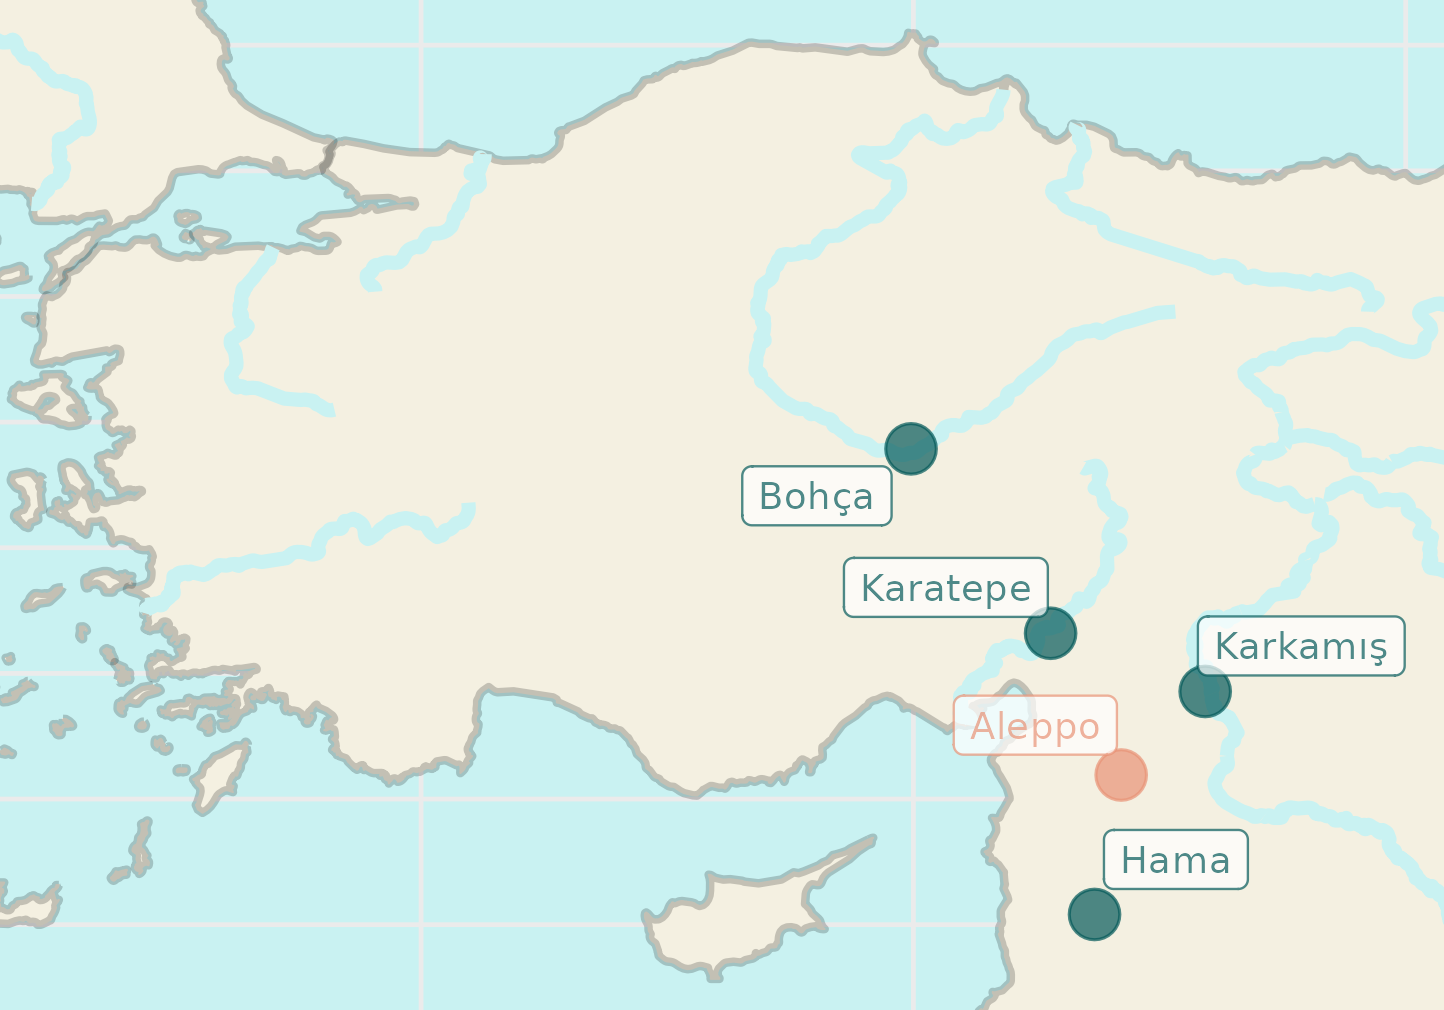
\includegraphics[width=.8\textwidth]{../../../Mídia/Map05.png}
\end{center}

% A inscrição de Karatepe faz referência à cidade da idade do ferro Adana, fenício
% \emph{ʾdn} (gentílico \emph{dnnym}), talvez equivalente ao país de Danuna
% mencionada pelas cartas de Amarna (em egípcio).
O sítio de Karatepe-Aslantaş (\autoref{fig:mapa_karatepe}) em si teria sido uma fortaleza no topo da colina,
cuja descoberta deve ser atribuída a Ekrem Kuşçu, professor de ensino
fundamental de Kadirli, que visitou o sítio quatro vezes nos anos de 1927 a
1944 e que em 1946 levou Helmuth Theodor Bossert e Halet Çambel para o sítio.
Bossert e Çambel publicam no mesmo ano um relatório preliminar sobre o sítio,
dando início às investigações. As escavações se iniciaram no ano seguinte sob
direção de Bossert e Bahadır Alkım.
Partes do bilíngue são publicadas entre os anos de 1948--74 por Bossert,
Steinherr, Meriggi, Güterbock, Gelb, Laroche e Hawkins e Morpurgo-Davies,
mas estas edições não são completas. Apenas em 1999, Halet
Çambel publica a versão final de Karatepe-Aslantaş (\citeabbrev*{CHLI2},
reproduzida em~\citeabbrev*{CHLI11} (pp.\ 45ff) e corrigida
em~\citeabbrev*{CHLI3} (pp.\ 178ff)).

\begin{figure}[h]
	\begin{center}
		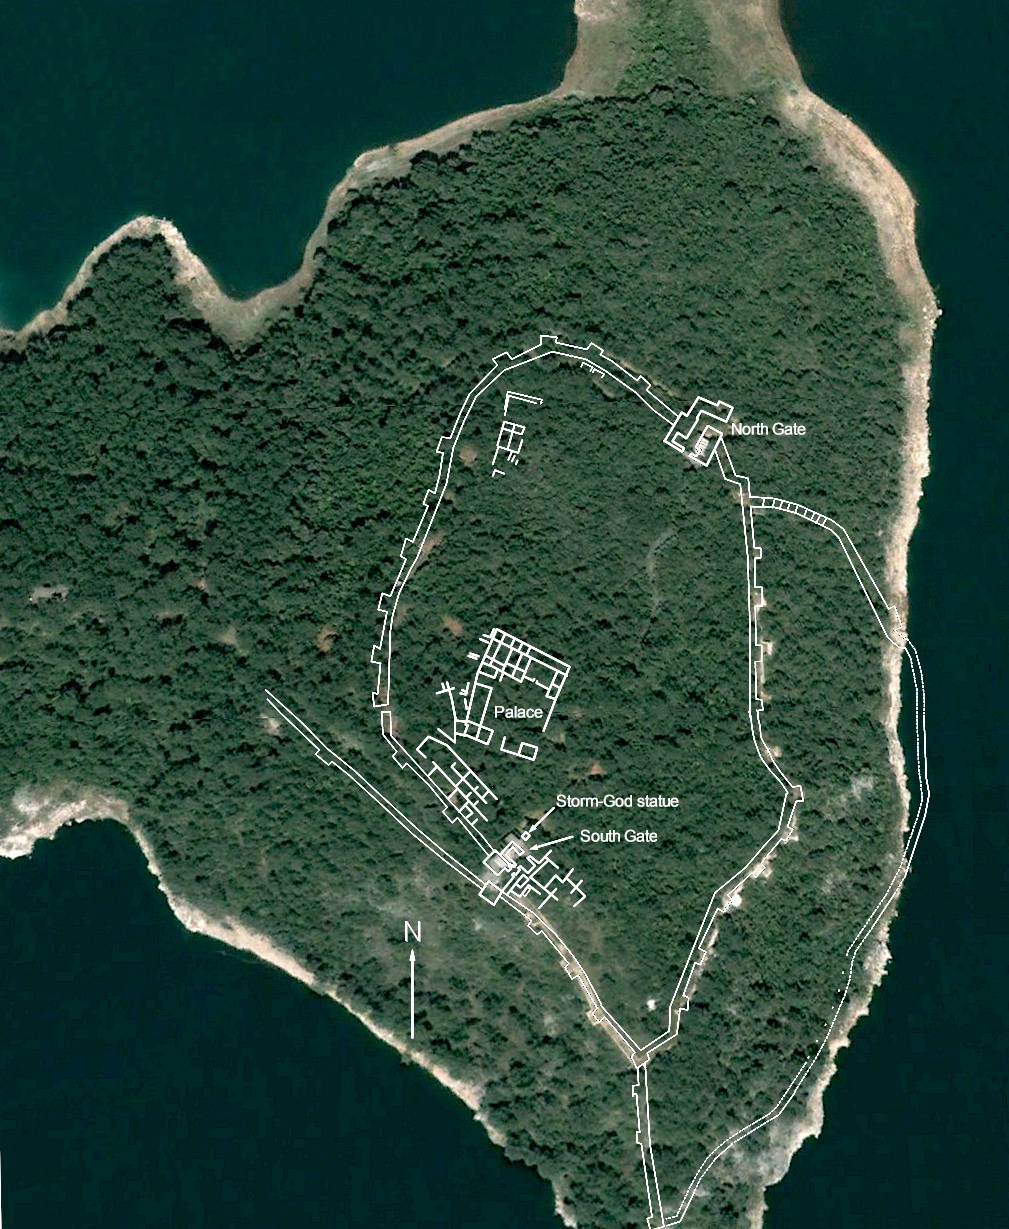
\includegraphics[width=0.9\textwidth]{../../../Mídia/karatepe0M2.jpg}
	\end{center}
	\caption[Mapa do sítio de Karatepe]{Mapa do sítio de Karatepe sobreposto na
		imagem de satélite do Google Maps.}\label{fig:mapa_karatepe}
\end{figure}


O bilíngue de Karatepe consiste em inscrições feitas nos muros de basalto dos
portões inferior (\emph{unten} > \emph{u}) e superior (\emph{oben} > \emph{o})
da fortificação.
Cada muro contém uma versão em luvita hieroglífico (\emph{H}) e uma em fenício
(\emph{Ph}), sendo assim as inscrições chamadas \emph{Hu.}, \emph{Ho.},
\emph{Phu.} e \emph{Pho.}.
Enquanto \emph{Hu.} e \emph{Phu.} estão preservadas praticamente por completo,
\emph{Ho.} e \emph{Pho.} estão em situação fragmentária.
As divergências entre \emph{Hu.} e \emph{Ho.} são mínimas.
As seis peças que constituem \emph{Hu.} foram descobertas parcialmente fora de
ordem, tendo sido reorganizadas a partir do texto fenício \emph{Phu.},
descoberto \emph{in situ}.
As inscrições fragmentárias \emph{Ho.} e \emph{Pho.} foram descobertas fora de
ordem e dependem da interpretação das versões do portão inferior.
Os ortostatos permanecem no sítio arqueológico, apenas reposicionados para
refletir sua distribuição original no espaço.

O texto é colocado na voz de Azatiwada, governante local que fora posto no cargo
por Awariku de Adana, possivelmente identificado com Urikki de Que (reino:
738--32 \textsc{aec}, ativo até 710--9), permitindo, junto a detalhes
paleográficos do fenício e dos hieróglifos, datar a inscrição do fim do século
VIII \textsc{aec}.
Azatiwada conta dos seus atos que favoreceram a cidade de Adana e Pahara,
institui alguns sacrifícios para Tarhunta, dedica a fortaleza a deuses
relacionados a grãos e vinícolas e faz uma maldição preventiva para proteger a
inscrição e seu nome.

\begin{figure}
	\begin{center}
		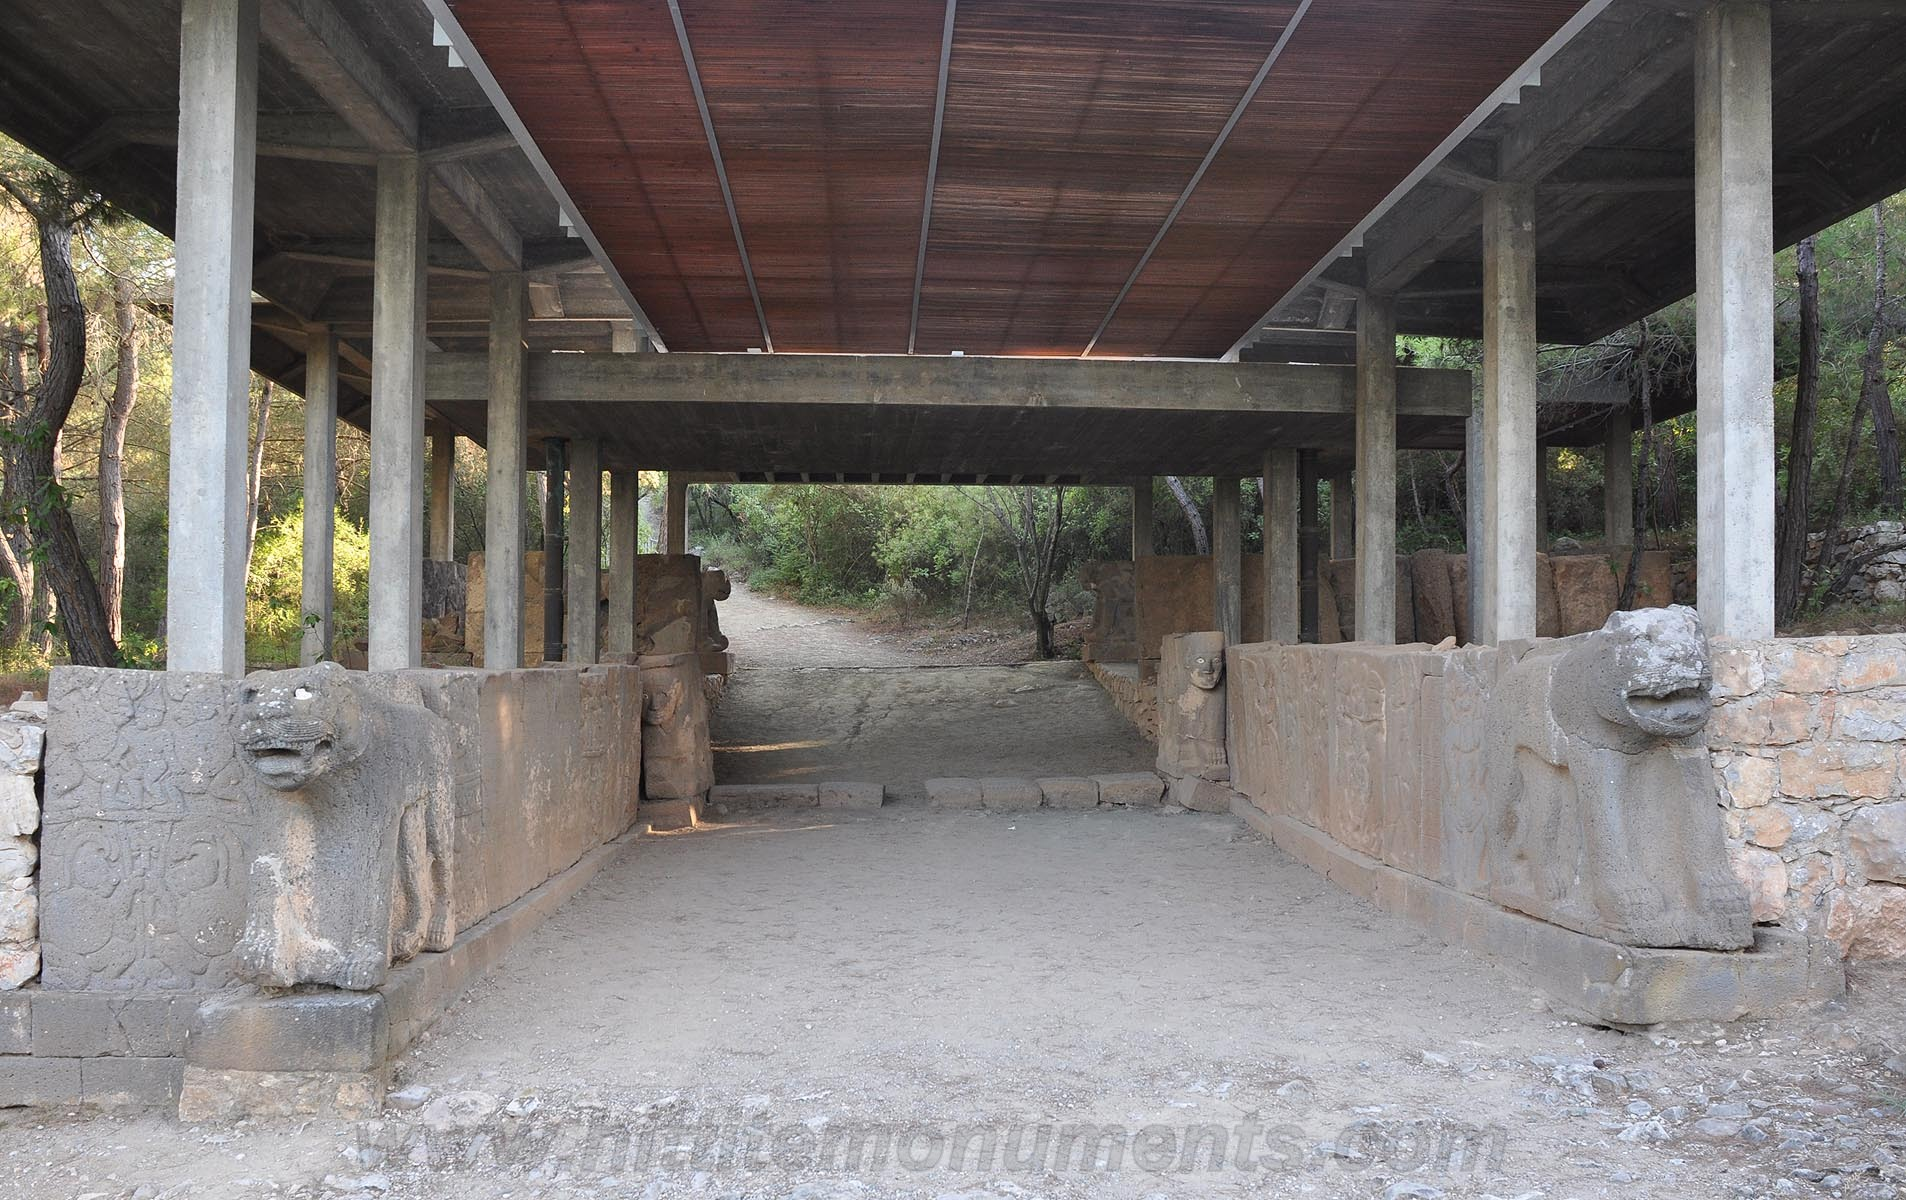
\includegraphics[width=\textwidth]{../../../Mídia/karatepe01.jpg}
	\end{center}
	\caption[Portão Inferior (Norte) de Karatepe]{Portão Inferior (Norte) de
		Karatepe.
		Imagem de Bora Bilgin, 2008, disponível em
		\href{https://www.hittitemonuments.com/karatepe}{Hittite Monuments}.
	}\label{fig:portaoU}
\end{figure}

\begin{figure}
	\begin{center}
		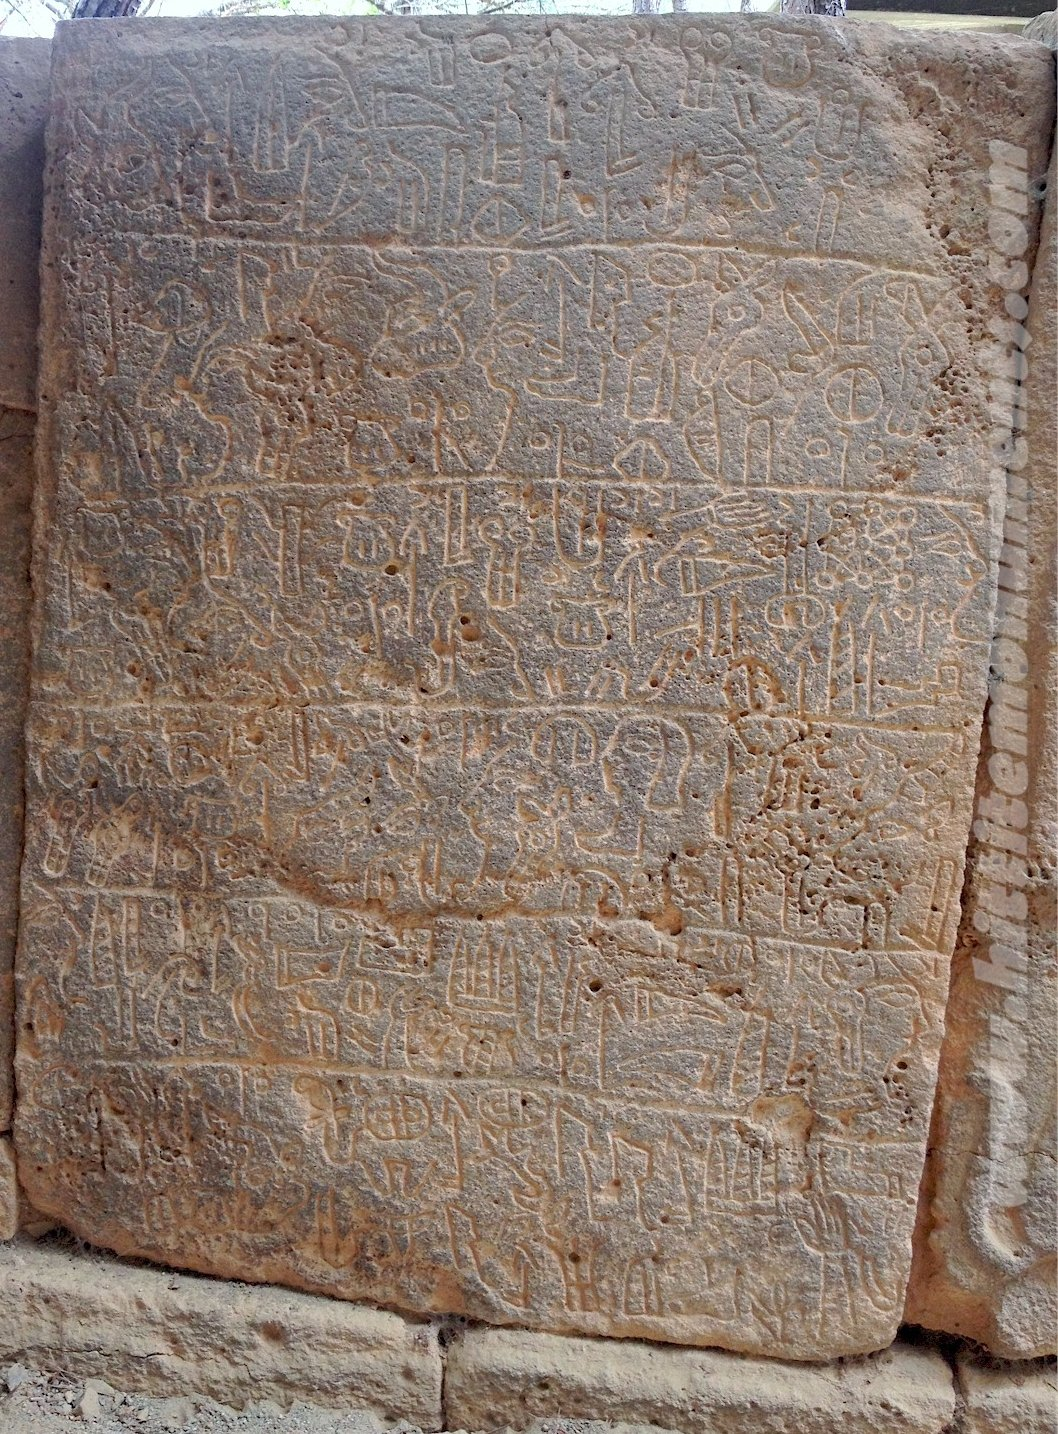
\includegraphics[width=0.95\textwidth]{../../../Mídia/karatepe58.jpg}
		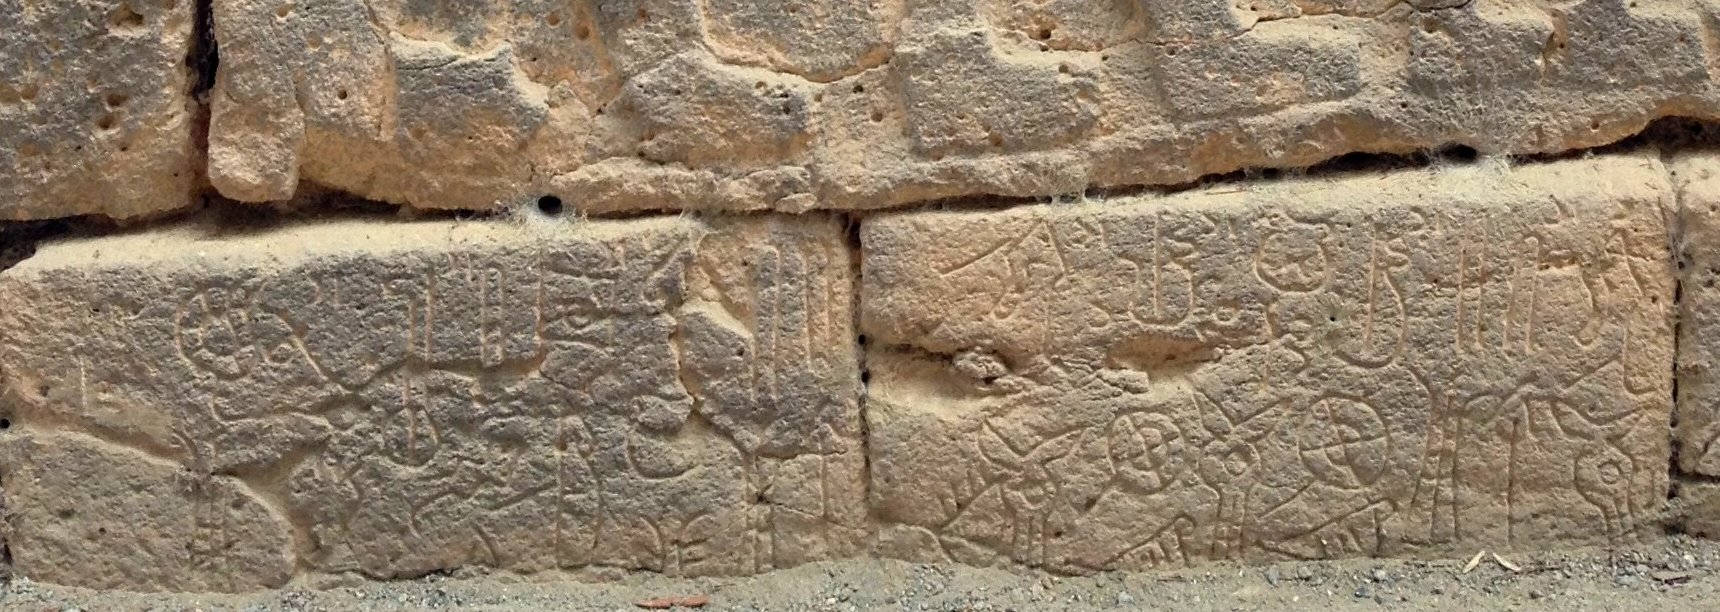
\includegraphics[width=0.95\textwidth]{../../../Mídia/karatepe104.jpg}
	\end{center}
	\caption[Ortostatos de Karatepe (Portão Inferior)]{Ortostatos de Karatepe
		(Portão Inferior).
		Imagens de Bora Bilgin, 2008, disponível em
		\href{https://www.hittitemonuments.com/karatepe}{Hittite Monuments}.
	}\label{fig:karatepe_a}
\end{figure}



\clearpage
\begin{parnumbersr}

	\raggedright%
	\itshape%

	\lmasc{}\logo{EGO}-mi
	\spac{}\logo{(LITUUS)}á-za-ti-i-wa/i-da-sá
	\logo{(DEUS)}\logo{SOL}-mi-sá
	\logo{(CAPUT)}-ti-i-sá
	\logo{(DEUS)}\logo{TONITRUS}-hu-ta-sa
	\logo{SERVUS}-la/i-sá

	á-wa/i+ra/i-ku-sa-wa/i
	\lbreak{}
	\logo{REL}-i-na
	\logo{MAGNUS}+ra/i-nu-wa-ta
	á-TANA-wa/i-ní-i-sá\logo{(URBS)}
	\logo{REX}-ti-sá

	wa/i-mu-u
	\logo{(DEUS).TONITRUS}-hu-za-sa á-TANA-wa/i-\emph{||}-ia\logo{(URBS)}
	\logo{MATER}-na-tí-na tá-ti-ha i-zi-i-da

	\lmasc{}\logo{ARHA}-ha-wa/i
	\lmasc{}la+ra/i+a-nú-ha
	\lmasc{}á-TANA-wa/i-na\logo{(URBS)}

	\lmasc{}\logo{(“MANUS”)}la-tara/i-ha-ha-wá/í
	\lmasc{}á-TANA-wá/í-za\logo{(URBS)} \lmasc{}\logo{“TERRA+X”}{(-)}wá/í+ra/i-za
	\lmasc{}zi-na \lmasc{}\logo{(“OCCIDENS”)}i-pa-mi \lmasc{}\logo{VERSUS}-ia-na
	\lmasc{}zi-pa-wá/í \logo{(ORIENS)}ki-sà-ta-mi-i \lmasc{}VERSUS-na

	\lmasc{}á-mi-ia-za-há-wa/i \logo{(“DIES<”>)}ha-lí-za
	\lmasc{}á-TANA-wá/í-ia\logo{(URBS)} \lmasc{}\logo{OMNIS+}MI-ma
	\logo{(“BONUS”)}sa-na-wa/i-ia \lmasc{}\logo{(“CORNU+RA/I”)}su+ra/i-sa
	\lmasc{}\logo{(LINGERE)}ha-sa-sa-ha á-sá-ta


	\lmasc{}\logo{(“MANUS”)}su-wá/í-ha-ha-wá/í
	\lmasc{}pa-há+ra/i-wa/i-ní-zi\logo{(URBS)}
	\lmasc{}\logo{(<“>*255”)}ka-ru-na-zi

	\lmasc{}\logo{EQUUS.ANIMA}-zú-ha-wa/i-ta \logo{(EQUUS.ANIMA)}á-zú-wa/i
	\lmasc{}\logo{SUPER}+ra/i-ta \lmasc{}i-zi-i-ha

	\logo{EXERCITUS}-lu/a/i-za-pa-wa/i-ta \lmasc{}\logo{EXERCITUS}-lu/a/i-ní
	\lmasc{}\logo{SUPER}+ra/i-ta \lmasc{}i-zi-i-há

	\lmasc{}\logo{(<“>SCUTUM”)}hara/i-li-pa-wa/i-ta
	\lmasc{}\logo{(“SCUTUM”)}hara/i-li \lmasc{}\logo{SUPER}+ra/i-ta
	\lmasc{}i-zi-i-há $[^\text{Ho.}$\ \logo{OMNIS-}MI-ma-za
					\lmasc{}\logo{{(DEUS)}TONITRUS}-hu-ta-tí \logo{DEUS}-na-ri+i-ha$]$


\end{parnumbersr}


\vspace{10pt}
\hrule
\vspace{10pt}


\setcounter{parcount}{0}
\begin{parnumbersr}

	\raggedright%
	\itshape%

	amu=mi Azatiwadas tiwadamis \logo{CAPUT}-tis Tarhunt{(a)}s hudarlis,

	Awarikus=wa \lbreak{} kwin uranuwata Adanawanis hantawatis,

	*a=wa=mu Tarhunz Adanawaya anatin tadin=ha izida.

	arha=ha=wa laranuha Adanawan.

	lataraha=ha=wa Adanawan=za walirin=za zin ipami tawiyan zin=pa=wa kistami
	tawiyan.

	amiyanza=ha=wa halinza Adanawaya tanima sanawiya \logo{(“CORNU+RA/I”)}-suras
	hasas=ha asta.

	suwaha=ha=wa Paharawaninzi karunanzi,

	azun=ha=wa=ta azuwi saranta iziha,

	kulanin=za=pa=wa kulani saranta iziha,

	haralin=pa=wa=ta harali saranta iziha, $[^\text{Ho.}$\ taniman=za Tarhuntadi masanari=ha$]$.


\end{parnumbersr}


\clearpage%
\noindent\textbf{Tradução}

[I] Eu sou Azatiwada, homem abençoado{(?)} pelo sol, servo de Tarhunta, [II] que
Awariku, rei de Adanawa, elevou, [III] e Tarhunta me fez da (cidade de)
Adanawa mãe e pai. [IV] Eu fiz (a cidade de) Adanawa prosperar, [V] eu estendi
a planície de Adanawa de um lado em direção ao ocidente, do outro em direção
ao oriente [VI] e, nos meus dias, havia em Adanawa todos os bens, abundância e
saciedade (\emph{ou} luxo). [VII] Eu enchi os celeiros de Pahara [VIII] e fiz
cavalo e mais cavalo, [IX] e fiz exército e mais exército, [X] e fiz escudo e
mais escudo, tudo por {(graça de?)} Tarhunta e pelos deuses (\emph{ou} pela
graça dos deuses).

\bigskip
\noindent\textbf{Notas}

\smallskip
\noindent\textbf{§I}\tabto{2em}
\textbf{\emph{tiwadamis}} `abençoado/a pelo deus Sol': o nome do deus Sol em
luvita é \emph{Tiwad{(a)}-}\footnote{Ver formas quase completas em KÜRTÜL, §6 e
	KARKAMIŠ A15\emph{b}, §1.} e esta forma utiliza o sufixo de formação de
adjetivos \emph{-ami-}.
O sentido específico deo adjetivo como \emph{abençoado/a} é gerado a partir do
fenício \emph{h-brk}.
\textbf{CAPUT-\emph{tis}} `pessoa, homem': a forma subjacente é incerta, nunca
sendo escrita em sua completude fonologicamente.
O termo \emph{ziti-} `homem' parece apenas ocorrer com L.313 𔕠 VIR, fazendo-nos
crer que L.10 𔐉 CAPUT é reservada para outro elemento semântico.
No entanto, em diversas passagens de KARATEPE, CAPUT\emph{-ti-} corresponde ao
fenício \emph{ʾdm} `homem'.
\textbf{\emph{hudarlis}} `servo': fonologia reconstruída a partir do
luvita cuneiforme \emph{hudarli-}.

\smallskip
\noindent\textbf{§II}\tabto{2em}
\textbf{\emph{Awarikus=wa kwin}}: oração relativa com o sujeito antecedendo o
pronome que recupera \emph{amu} `eu' de §1. Awariku foi por vezes
identificado com o rei Urikki de Que, tributário de Tiglate-pileser III\@,
mas a evidência é pouca e há a possibilidade de ser o avô deste.

\smallskip
\noindent\textbf{§III}\tabto{2em}
\textbf{\emph{Tarhunz}} `Tarhunta': a divindade Tarhunta no texto fenício é
traduzida como \emph{bʿl} `Baal \slash{} senhor'.
A variação das formas \emph{\logo{{(DEUS)}TONITRUS}-hu-ta-sa} e
\emph{\logo{{(DEUS)}TONITRUS}-hu-za} talvez indique que o nome da divindade fosse
um tema consonantal em \emph{-t}, \emph{Tarhunt-}, com o nominativo
\emph{Tarhunz} \ipa{/tar.hunts/}, o mesmo valendo para a divindade solar Tiwad,
cujo nominativo seria \emph{Tiwaz} \ipa{/ti.wats/}.
\textbf{\emph{\emph{MATER}-na-tí-na}} `mãe': a leitura é garantida pelo fenício
\emph{ʾm} `mãe', pois a partir da grafia luvita, tanto \emph{anatin} `mãe'
quanto \emph{wanatin} `mulher' poderiam ser interpretados, uma vez que L.79 𔑘
FEMINA\slash{}MATER é utilizado para ambos os temas e ambos são temas em
\emph{-n-} sufixadas pelo morfema \emph{-ati-}.

\smallskip
\noindent\textbf{§IV}\tabto{2em}
\textbf{\emph{ARHA} {=?} \emph{arha-/aha-}} `completamente': é incerto se o
prevébio e advérbio representado por L.216 𔓸 ARHA era fonologicamente realizado
com a sequência \ipa{/rh/} ou com a sequência \ipa{/hh/} produzida por
assimilação, \emph{vide} hit.\ \emph{\hittitetrans{arha}} mas luv.cun.
\emph{\hittitetrans{ahha}}. Para uma discussão das formas,
ver~\citet{Yakubovich2012}.
\textbf{\emph{la+ra/i+a-nú-ha} {=?} \emph{laranuha}} `fazer prosperar?': talvez
seja uma forma causativa do verbo \emph{lada-\slash{}lara-} atestado em
AKSARAY, §2 e SULTANHAN, §6. O sentido é produzido a partir da comparação com o
hit.\ \emph{lazziya-} `prosperar', embora não esteja clara a fonologia.
A passagem em fenício contém \emph{ḥw} `fazer viver'.
Ver mais em~\citet[104--5]{HawkinsMorpurgo1978}.

\smallskip
\noindent\textbf{§V}\tabto{2em}
\textbf{\emph{\emph{“TERRA+X”}{(-)}wá/í+ra/i-za} {=?} walirin=za} `planície':
para discussão sobre a forma subjacente e troca da forma esperada
\emph{walili{(da)}-} por \emph{waliri{(da)}-},
ver~\citet[106]{HawkinsMorpurgo1978}, que também sugerem a possibilidade de
uma haplologia, i.e. *\emph{walirin=za} >
\emph{warin=za}, ou de haplografia, i.e.\ \luwiantrans{wá-ra-ra-za}
\emph{wá/í+ra/i-ra/i-za} > \luwiantrans{wá-ra-za} \emph{wá/í+ra/i-ra/i-za}.
Possível correlato de hit.\ \emph{ulili-} `campo'.
O sentido de `planície' é dado pelo fenício
\emph{ʿmq} `vale, planície'.
\textbf{\emph{zin\ldots{} zin=pa}} `de um lado\ldots{} do outro': o
ablativo-instrumental \emph{zin} tem o sentido de `aqui', a construção
contrastiva \emph{zin\ldots{} zin{(=pa)}} é comum para denotar `por um
lado\ldots{} por outro', no sentido local mas também lógico.


\smallskip
\noindent\textbf{§VI}\tabto{2em}
\textbf{\emph{tanima}} `todas': neutro plural de \emph{tanima-}, a forma neutra
plural em \emph{-aya} aparece em Ho.\ §XV\@.
\textbf{\emph{sanawiya}} `(coisas) boas = bens': neutro com sentido abstrato. A
interpretação da forma talvez seja \emph{sana-awi-} `bem-vindo', \emph{vide}
\citet{YakubovichWelcome}. Em fenício temos \emph{nʿm} `bens'.
\textbf{\emph{\emph{(“CORNU+RA/I”)}su+ra/i-sa} {=?} \emph{suras}} `abundância':
a forma subjacente não é cla\-ra, mas possivelmente esteja associada ao verbo
\emph{suwa-} `encher, preencher' (hit.\ \emph{suwai-}). A forma fenícia oferece o
sentido, \emph{šbʿ} `abundância'.
\textbf{\emph{\emph{(LINGERE)}ha-sa-sa} {=?} \emph{hasas}} `saciedade': a forma
subjacente é incerta, mas possivel\-mente seja um homônimo de \emph{hasa-} `força'
(KARKAMIŠ A11b+c, §30), que, no entanto, é acompanhada do logograma L.314 𔕡.
O logograma L.112 𔒈 LINGERE é sempre complementado por \emph{ha/há-sa/sá} e tem
o sentido de `saciedade' ou `luxo'.
O texto fenício apresenta \emph{mnʿm} `luxo'.

\smallskip
\noindent\textbf{§VIII-X}\tabto{4em}
\textbf{\emph{azun\slash{}kulanin\slash{}haralin\ldots{}
		azuwi\slash{}kulani\slash{}harali saranta}}
`cavalo\slash{}exér\-ci\-to\slash{}escudo sobre cavalo\slash{}exército\slash{}escudo':
literalmente, as frases significam `eu fiz X sobre X', mas o sentido parece ser
de acúmulo `eu fiz X e mais X'.
Note-se que o texto fenício inverte a ordem de \emph{exército} e \emph{escudo},
Phoen. §IX \emph{mgn} `escudo' e §X \emph{mḥnt} `exército'.
O mesmo ocorre na versão hieroglífica Ho.

\smallskip
\noindent\textbf{§IX}\tabto{2em}
\textbf{\emph{\emph{EXERCITUS}-lu/a/i-za} {=?} \emph{kulanin=za}} `exército': se
aceitarmos que a for\-ma é idêntica ao luv.cun. \emph{kulana} (hit.
\emph{kuwalana-}), a melhor transliteração seria
\emph{\emph{EXERCITUS}+LU/A/I-za}, indicando que \emph{lu/a/i} age como
desambiguador fonológico e não se grafou a fonologia completa do termo.
Há também a possibilidade de se interpretar a forma subjacente como um tema em
nasal \emph{kulan-}, reforçado pela forma de ablativo
\emph{\emph{EXERCITUS}-lu/a/i-na-ti-i} {=?} \emph{kulanadi} (TELL AHMAR 6,
§24).

\smallskip
\noindent\textbf{§X}\tabto{2em}
\textbf{\emph{\emph{OMNIS}-MI-ma-za\ldots{} \emph{DEUS}-na-ri+i-ha}}: este trecho
está danificado em Hu., tendo sido reconstruído a partir da versão hieroglífica Ho.

\clearpage
\setcounter{parcount}{10}
\begin{parnumbersr}

	\raggedright%
	\itshape%


	\logo{REL}-pa-wá/í \lmasc{}\logo{(*255)}mara/i\textsuperscript{+ra/i}-ia-ní-zi
	\lmasc{}\logo{ARHA} \lmasc{}ma-ki-sa\textsuperscript{!}-há \lmasc{}\lmasc{}


	\lmasc{}\logo{(“MALUS2”)}ha-ní-ia-ta-<ia>-pa-wa/i-ta-a \lmasc{}\logo{REL}-ia
	\lmasc{}\logo{(TERRA)}ta-sà-REL+ra/i \lmasc{}a-ta \lmasc{}á-sá-ta


	\lmasc{}wá/í-ta \logo{(TERRA)}ta-sà-\logo{REL}+ra/i<-ri+i>
	\logo{ARHA} \lmasc{}\textsc{⌈}\logo{*501}\textsc{⌉} $[$…$]$-há

	\lmasc{}á-ma\lmasc{}\lmasc{}-za\textsubscript{4}-há-wá/í-ta
	\lmasc{}\logo{DOMINUS}-ní-za
	\lmasc{}\logo{DOMUS}-na-za \lmasc{}\logo{(BONUS)}sa-na-wá/í
	\lmasc{}u-sa-nú-há

	\lmasc{}á-mi-há-wa/i \lmasc{}\logo{DOMINUS}-ní-i
	\lmasc{}\logo{(NEPOS)}ha-su-a \lmasc{}\logo{OMNIS}-MI-ma
	\lmasc{}\lmasc{} \logo{(BONUS)}sa-na-wa/i-ia
	\lmasc{}\logo{CUM}-na i-zi-i-há

	\lmasc{}á-pa-sá-há-wá/í-ta \lmasc{}tá-ti-i
	\lmasc{}\logo{(“THRONUS”)}i-sà-tara/i-ti
	\lmasc{}\logo{(“SOLIUM”)}$[$i$]$-s$[$à-nu-wa/i-ha$]$

	$[$\ldots$]$

	$[$\lmasc{}\logo{OMNIS}-MI-sa-ha-wa/i-mu-ti-i \logo{REX}-ti-sa
					\lmasc{}tá-ti-na$]$ \lmasc{}$[$i-zi$]$-i-$[$da$]$
	\lmasc{}á-$[$mi$]$-ia-ti
	\lmasc{}\logo{IUSTITIA}-na-ti \lmasc{}á-mi-ia+ra/i-ha
	\lmasc{}\logo{(“COR”)}á-ta-na-sa-ma-ti \lmasc{}á-mi-ia+ra/i-há
	\lmasc{}\lmasc{} \lmasc{}\logo{(“BONUS”)}sa-na-wa/i-sa-tara/i-ti



\end{parnumbersr}

\vspace{10pt}
\hrule
\vspace{10pt}

\setcounter{parcount}{10}
\begin{parnumbersr}

	\raggedright%
	\itshape%

	kwipa=wa mariyaninzi arha makisaha,

	haniyataya=pa=wa=ta kwiya taskwiri anta asanta,

	a=wa=ta taskwirari arha parhaha.

	aman=za=ha=wa nanin=za parnan=za sanawi usanuha.

	ami=ha=wa nani \logo{NEPOS}-hasu{(w)}a tanima sanawaya \logo{CUM}-na iziha

	apas=ha=wa=ta tadi isatarati isanuwaha.

	$[$\ldots{}$]$

	tanimis=ha=wa=mu=ti hantawatis tadin izida amiyadi tarawanadi amiyari=ha
	atnasamadi amiyari=ha sanawastradi.

\end{parnumbersr}

\bigskip%
\noindent\textbf{Tradução}

[11] De fato fiz acumularem muito as colheitas dos campos-\emph{mariyana-}, [12]
enquanto os males que haviam na terra [13] eu os afastei completamente da terra.
	[14] e a casa do meu senhor eu abençoei bem, [15] e fiz todos bens para a
descendência{(?)} do meu senhor, [16] e fi{(-la)} sentar no trono de seu pai. [17]
\ldots{} [18] Todo rei me fez para si seu pai pela minha justiça e pela minha
sabedoria e pela minha bondade.

\bigskip
\noindent\textbf{Notas}

\smallskip
\noindent\textbf{§XI}\tabto{2em}
\textbf{\emph{mariyaninzi\ldots{} makisaha}} `acumulei
colheitas dos campos-\emph{mariyana}': a interpretação dessa passagem
é difícil, em parte pela presença de \emph{hapax legomena} tanto no texto luvita
quanto no texto fenício.
Sigo aqui a interpretação de \citet{VanDenHout2010}:
\textbf{\emph{mariyaninzi}}: ligada ao hitita
\textsuperscript{A.ŠÀ}\emph{mariyana-} `tipo de
campo? campo de um vegetal específico?' (KBo 10.37 12-17, 21-26), bem como às
formas luv.hier. \emph{mara/iwali-} `vegetação útil? centeio?' (SULTANHAN §6),
hit. \emph{marawalliya/i-} `campo de grãos', utilizando como evidência o uso de
L.255 𔔡 como determinativo de \emph{karunanzi} `silos (de grãos)' nesta
inscrição;
a forma escrita no texto, \emph{mariyaninzi}, deve ser interpretada como uma
forma contrata de *\emph{mariyaniyinzi}, contração da sequência \emph{-iyi-},
comum em luvita.
\textbf{\emph{makisaha}}: ligada ao hitita \emph{mekki-} `muito, numeroso' e à
passagem \emph{nu=kan ḫalkiuš EGIR-an maknunun} `eu fiz as colheitas (serem)
abundantes novamente' (Proclamação de Telipinu, KBo 3.1 iii 44, KUB 11.1 iii 8,
KBo 3.67 iii 1 + KUB 31.17:5).
Em resumo, a forma hipotética \emph{mariyaniyi-} significaria `relativo aos
campos do tipo \emph{mariyana-} > colheitas do campo-\emph{mariyana-}?' e o
verbo \emph{makisa-} seria uma forma iterativa de um verbo \emph{maki-} `fazer
crescer/abundante'.


\smallskip
\noindent\textbf{§XII}\tabto{2em}
\textbf{\emph{\emph{(“MALUS2”)}ha-ní-ia-ta-<ia>}} `males': o texto da versão
luvita Hu.\ parece ter ignorado um grafema, <\emph{ia}>, suplementado por conta
da versão Ho.\ e do pronome relativo \emph{kwiya} (nom.neut.pl.).

\smallskip
\noindent\textbf{§XIV}\tabto{2em}
\textbf{\emph{usanuwa}} `abençoar': literalmente, o verbo \emph{usanu{(wa)}-}
seria um causativo do verbo \emph{wasa-} `ser bom', logo `fazer ser
bom'. O sentido de abençoar neste contexto foi proposto pelo fato de que ao
longo do bilíngue, o fenício \emph{brk} `abençoar' é utilizado para traduzir
formas do verbo \emph{usanu{(wa)}-}.
No entanto, o texto fenício neste contexto contém o verbo \emph{yṭnʾ} `eu
ergui', o que suscitou as tentativa de interpretar \emph{usanu-} como um tema
cognato do hitita \emph{wete-} `construir', mas isso produziria um \emph{hapax
	legomena}.

\smallskip
\noindent\textbf{§XV}\tabto{2em}
\textbf{\emph{\emph{NEPOS}-hasu{(w)}a}} `descendência?': incerto, mas deve ser
um dativo singular comum.




\clearpage
\setcounter{parcount}{18}
\begin{parnumbersr}

	\raggedright%
	\itshape%

	\logo{(“CASTRUM”)}ha+ra/i-ní-sà-pa-wá/í \lmasc{}\logo{(PUGNUS)}lu/a/i-mi-da-ia
	\textsc{⌈}\logo{AEDIFICARE}\textsc{⌉}-MI-ha
	$[$\ldots$]$ $[^\text{Ho.}$\ \lmasc{}\logo{(“FINES”)}i+ra/i-há-za $]$

	\logo{(MALUS)}á-tu-wa/i-ri+i-zi-wa/i-ta
	\lmasc{}\logo{CAPUT}-tí-zi \lmasc{}\logo{REL}-ta-na \lmasc{}a-ta \textsc{⌈}á-sa-ta\textsc{⌉}
	\logo{(\textsc{⌈}“*217\textsuperscript{?}\textsc{⌉}”)}u-sa-lí-\textsc{⌈}zi\textsc{⌉}

	\logo{NEG\textsubscript{2}}-wá/í \logo{REL}-zi \lmasc{}SUB-na-na \logo{PUGNUS.PUGNUS}-la/i-ta
	\lmasc{}mu-ka-sa-sa-na \lmasc{}\logo{DOMUS}-ní-i

	á-mu-pa-wá/í-ma-da \lmasc{}\logo{(LITUUS)}á-za-ti-wa/i+ra/i-sá
	\lmasc{}\logo{(“PES”)}pa-da-za \lmasc{}\logo{SUB}-na-na
	\lmasc{}\logo{PONERE}-há

	\lmasc{}\logo{REL}-pa-wá/í-ta \logo{LOCUS}-la/i-ta-za-'
	\lmasc{}á-pa-ta-za \lmasc{}\logo{(“CASTRUM”)}ha+ra/i-ní-sà \lmasc{}a-ta
	\lmasc{}\logo{AEDIFICARE+}MI-ha

	\lmasc{}á-TANA-wa/i-sa-wa/i\logo{(URBS)} \lmasc{}\lmasc{} \lmasc{}\logo{REL}-ti
	\lmasc{}\logo{(BONUS)}wa/i+ra/i-ia-ma-la \lmasc{}\logo{SOLIUM}-MI-i

	\lmasc{}\logo{*274}-ta-li-ha-há-wa/i \logo{“CASTRUM”}-sà
	\logo{(PUGNUS)}lu/a/i-mi-da-ia-a \lmasc{}\lmasc{} \logo{(“OCCIDENS”)}i-pa-mi
	\logo{“VERSUS”}-na

	\lmasc{}\logo{NEG\textsubscript{2}}-wa/i \logo{REL}-ia \logo{(L.274)}ha-ta-la-i-ta
	\lmasc{}\logo{FRONS}-li-zi \logo{REX}-ti-zi

	\lmasc{}á-mu \lmasc{}\lmasc{} \logo{REL}-zi \lmasc{}\logo{PRAE}-na \lmasc{}á-sá-ta


\end{parnumbersr}

\vspace{10pt}
\hrule
\vspace{10pt}

\setcounter{parcount}{18}
\begin{parnumbersr}

	\raggedright%
	\itshape%

	harnisan=pa=wa \logo{PUGNUS}-lumidaya tamaha $[$\ldots{}$]$ irhanza.

	atuwarinzi=wa=ta \logo{CAPUT}-tinzi kwitan anta asanta, usalinzi,

	na=wa kwinzi anan hudarlainta Muksasan parni,

	amu=pa=wa=mw=ada, Azatiwaras, padanza anan tuwaha.

	kwipa=wa=ta arlantanza apatanza harnisa anta tamaha,

	Adawanas=wa kwati warayamala asai.

	hataliha=ha=wa  harnisa \logo{PUGNUS}-lumidaya ipami tawiyan,

	na=wa kwiya hatalainta hantilinzi hantawatinzi,

	amu=wa kwinzi paran asanta.

\end{parnumbersr}

\bigskip%
\noindent\textbf{Tradução}

[19] E forte fortaleza eu construí [\ldots] nas fronteiras. [20] Onde quer que
houvesse más pessoas, ladrões [21] que não haviam servido sob a
casa de Muksa, [22] eu mesmo, Azatiwada, os coloquei sob meus pés. [23] De
fato eu construí naqueles territórios a fortaleza, [24] para que Adana ficasse
em paz. [25] Eu esmaguei fortes fortalezas em direção ao oeste, [26] as quais
não haviam esmagado os reis anteriores, [27] que vieram antes de mim.

\bigskip
\noindent\textbf{Notas}

\smallskip
\noindent\textbf{§XIX}\tabto{3em}
\textbf{\emph{\emph{PUGNUS}-lu/a/i-mi-da-}} `forte': a leitura permanece
incerta. O sentido é confirmado pelo fenício \emph{ʿz}.

\smallskip
\noindent\textbf{§XX}\tabto{3em}
\textbf{\emph{usalinzi}} `ladrões': forma produzida pelo radical verbal
\emph{usa-} `trazer', o sentido, no entanto, não é confirmado pelo fenício.
O determinativo L.217 𔓺 não é compreendido.

\smallskip
\noindent\textbf{§XXI}\tabto{3em}
\textbf{\emph{\emph{PUGNUS.PUGNUS}-la/i-ta} {=?} hudarlainta} `serviram':
Sigo a leitura de~\citet{RiekenYakubovich2010}, mantendo que o sentido
dado pelo fenício \emph{ʿbd kn} `servir, ser servo de' é adequado.
No entanto, ver~\citet{MelchertPugnus}.
\textbf{\emph{Muksasan}} `de Muksa': associa-se a figura de Muksa, no fenício,
\emph{MPŠ} ao herói lendário grego Mopso/Mokso, talvez também em hit.\
\emph{Muksu}. A forma é um dativo singular do adjetivo de posse (com a
desinência peculia \emph{-an}).

\smallskip
\noindent\textbf{§XXIII}\tabto{3em}
\textbf{\emph{arlantanza}} `nos lugares': *\emph{arla-} `lugar' tem sido
revisado para \emph{arlant-} por conta das formas de dativo com \emph{-ta-za} ou
\emph{-da-da-za}, \emph{vide}~\citet{Yakubovich2017}.


\bigskip
\begin{multicols}{2}[\noindent\textbf{Vocabulário}]
	\begin{hangparas}{1em}{1}
		\raggedright%
		\textbf{\emph{Adanawan{(a)}-}} (\emph{adj.}) \tabto{1em} relativo a Adana\\
		\textbf{\emph{anan}} (\emph{prev.}) \tabto{1em} sob,abaixo\\
		\textbf{\emph{anati-}} (\emph{subst.com.}) \tabto{1em} mulher\\
		\textbf{\emph{arlant-}} (\emph{subst.neut.}) \tabto{1em} lugar\\
		\textbf{\emph{asa-}} (\emph{v.i.}) \tabto{1em} sentar,estar\\
		\textbf{\emph{atnasama-}} (\emph{subst.}) \tabto{1em} sabedoria\\
		\textbf{\emph{atuwal{(i)}-}} (\emph{adj.}) \tabto{1em} mau\\
		\textbf{\emph{Awariku-}} (NP) \tabto{1em} Awariku\\
		\textbf{\emph{Azatiwada-}} (NP) \tabto{1em} Azatiwada\\
		\textbf{\emph{azu-}} (\emph{subst.com.}) \tabto{1em} cavalo\\
		\textbf{\emph{\emph{CAPUT}-ti-}} (\emph{subst.com.}) \tabto{1em} pessoa,homem\\
		\textbf{\emph{\emph{(“CORNU+RA/I”)}-suras}} (\emph{subst.neut.}) \tabto{1em} abundância\\
		\textbf{\emph{hali-}} (\emph{subst.neut.}) \tabto{1em} dia\\
		\textbf{\emph{haniyata-}} (\emph{subst.com.}) \tabto{1em} mal\\
		\textbf{\emph{hantawati-}} (\emph{subst.com.}) \tabto{1em} rei\\
		\textbf{\emph{hantili-}} (\emph{adj.}) \tabto{1em} anterior,primeiro\\
		\textbf{\emph{harali-}} (\emph{subst.com.}) \tabto{1em}
		escudo\\\columnbreak%
		\textbf{\emph{harnisa-}} (\emph{subst.neut.}) \tabto{1em} fortaleza\\
		\textbf{\emph{hasa-}} (\emph{subst.}) \tabto{1em} luxo\\
		\textbf{\emph{hatal{(a)}i-}} (\emph{v.t.}) \tabto{1em} bater, acertar, golpear\\
		\textbf{\emph{hudarl{(a)}i-}} (\emph{v.i.}) \tabto{1em} servir\\
		\textbf{\emph{hudarli-}} (\emph{subst.}) \tabto{1em} servo\\
		\textbf{\emph{irha-}} (\emph{subst.com.}) \tabto{1em} fronteira\\
		\textbf{\emph{isanuwa-}} (\emph{v.t.}) \tabto{1em} sentar algo/alguém\\
		\textbf{\emph{isatarata-}} (\emph{subst.neut.}) \tabto{1em} trono\\
		\textbf{\emph{karuna-}} (\emph{subst.neut.}) \tabto{1em} celeiro\\
		\textbf{\emph{kulani-}} (\emph{subst.}) \tabto{1em} exército\\
		\textbf{\emph{ladanu-}} (\emph{v.t.}) \tabto{1em} fazer prosperar\\
		\textbf{\emph{latara-}} (\emph{v.t.}) \tabto{1em} estender\\
		\textbf{\emph{makisa-}} (\emph{v.t.}) \tabto{1em} acumular?\\
		\textbf{\emph{mariyani-}} (\emph{adj./subst.com.}) \tabto{1em} relativo aos campos-\emph{mariyana-}?\\
		\textbf{\emph{masani-}} (\emph{subst.com.}) \tabto{1em} deus\\
		\textbf{\emph{Muksa-}} (NP) \tabto{1em} Muksa\\
		\textbf{\emph{Muksasa-}} (\emph{adj.poss.}) \tabto{1em} de Muksa\\\columnbreak%
		\textbf{\emph{nani-}} (\emph{subst.com.}) \tabto{1em} senhor\\
		\textbf{\emph{nani(ya)-}} (\emph{adj.}) \tabto{1em} pertencente ao senhor\\
		\textbf{\emph{\emph{NEPOS}-hasu-}} (\emph{subst.com.}) \tabto{1em} descendência?\\
		\textbf{\emph{pada-}} (\emph{subst.}) \tabto{1em} pé\\
		\textbf{\emph{Paharawan{(a)}-}} (\emph{adj.}) \tabto{1em} relativo a Pahara\\
		\textbf{\emph{parha-}} (\emph{v.t.}) \tabto{1em} afastar\\
		\textbf{\emph{parna-}} (\emph{subst.}) \tabto{1em} casa\\
		\textbf{\emph{\emph{PUGNUS}-lumida-}} (\emph{adj.}) \tabto{1em} forte\\
		\textbf{\emph{sanawastra-}} (\emph{subst.}) \tabto{1em} bondade\\
		\textbf{\emph{sanawa/i-}} (\emph{adj.}) \tabto{1em} bom\\
		\textbf{\emph{sanawi}} (\emph{adv.}) \tabto{1em} bem\\
		\textbf{\emph{saranta}} (\emph{posp.}) \tabto{1em} em cima de\\
		\textbf{\emph{suwa-}} (\emph{v.t.}) \tabto{1em} encher, preencher\\
		\textbf{\emph{tadi-}} (\emph{subst.}) \tabto{1em} pai\\
		\textbf{\emph{tama-}} (\emph{v.t.}) \tabto{1em} construir\\
		\textbf{\emph{tanimi/a-}} (\emph{adj.}) \tabto{1em} todo\\
		\textbf{\emph{tarawana-}} (\emph{subst.}) \tabto{1em} justiça\\
		\textbf{\emph{taskwira/i-}} (\emph{subst.}) \tabto{1em} território\\
		\textbf{\emph{tawiyan}} (\emph{posp.}) \tabto{1em} até\\
		\textbf{\emph{tiwadami-}} (\emph{adj.}) \tabto{1em} abençoado por Tiwad\\
		\textbf{\emph{tuwa-}} (\emph{v.t.}) \tabto{1em} colocar\\
		\textbf{\emph{uranuwa-}} (\emph{v.t.}) \tabto{1em} fazer grande, elevar\\
		\textbf{\emph{usali-}} (\emph{subst.}) \tabto{1em} ladrão\\
		\textbf{\emph{usanu-}} (\emph{v.t.}) \tabto{1em} fazer bem? abençoar?\\
		\textbf{\emph{walili-}} (\emph{subst.}) \tabto{1em} campo, planície\\
		\textbf{\emph{warayamala}} (\emph{adv.}) \tabto{1em} em paz\\
	\end{hangparas}
\end{multicols}
